\section{Attention mechanism}
\label{appendix:attention}

Attention mechanisms, introduced in the Transformer paper \cite{transformer}, are pivotal in modern deep learning. This section explores the core components of transformers and their role in image and video synthesis models.






\subsection{Self-attention}

Self-attention allows us to model the weight of different parts of an input sequence. It gives indication on how much focus (\textbf{attention score}) to give to different elements in the sequence, and considers relationships between then. In self-attention, the same set of data elements provides the queries, keys and values, unlike cross-attention where we have two different sets of data elements.

\textbf{Input}: A vector $X \in \mathbb{R}^{n \times d}$.

\textbf{Output}: Similarity score between the elements in the sequence (equation \ref{eq:self_attention}).

\textbf{The Q, K, V matrices}: The Q, K, V matrices are learnable matrices that are used to calculate the attention scores. We can think of \textbf{Q}uery, \textbf{K}ey, \textbf{V}alue as text search in Google. When we \textit{query} Google, we get \textit{keys} as a result (list of pages), which is not what we are looking for. When we click on a page, then we get the \textit{value}. Therefor Google has to find similarity (attention scores) between query and the keys.

\textbf{Linear projection}: To get the Q, K, V matrices we apply linear projections on the input sequence $X$: 

\begin{align*}
    Q = X\cdot W_Q \\
    K = X\cdot W_K \\
    V = X\cdot W_V
\end{align*}

where $W_Q, W_K, W_V \in \mathbb{R}^{d \times d}$ are learnable weight matrices (they are assigned random values initially and learned during training).



\textbf{Cosine similarity}: We can think of similarity in linear algebra as cosine similarity between vectors $A, B$: 

\[ \text{CosSim} (A, B) = \frac{A \cdot B}{||A||\cdot ||B||} \]

Finally, the self-attention is defined as:

\begin{equation}
    \text{Attention}(Q, K, V) = \text{softmax}\left( \frac{QK^T}{\sqrt{d_k}} \right) V
    \label{eq:self_attention}
\end{equation}

where $d_k$ is the dimension of the key vector, and dividing by $\sqrt{d_k}$ normalizes the large magnitude of the dot product - which stabilizes the gradients and the training.

We then apply softmax function (see appendix \ref{appendix:activations}) to the attention weights, which converts the vector to a probability distribution between 0 and 1, which gives probability to tokens in the sequence. 

We then multiply (dot product) the attention weights with the value matrix to get the output. $K$ is transposed to match the dimensions of $Q$ (so we can multiply them).

\begin{lstlisting}[language=Python, breaklines=true, caption={Full implementation of a single self-attention block.}]
class SelfAttention(nn.Module):
"""
embed_dim (int): The dimensionality of the input embeddings.
attention_dim (int): The dimensionality of the attention space / attention vectors (Q, K, V).
"""
def __init__(self, embed_dim, attention_dim):
    super(SelfAttention, self).__init__()
    # Linear projections for Q, K, V
    self.W_Q = nn.Linear(embed_dim, attention_dim)
    self.W_K = nn.Linear(embed_dim, attention_dim)
    self.W_V = nn.Linear(embed_dim, attention_dim)
    self.scale = torch.sqrt(torch.tensor(attention_dim, dtype=torch.float32))

def forward(self, X):
    Q = self.W_Q(X)
    K = self.W_K(X)
    V = self.W_V(X)

    attention_scores = torch.matmul(Q, K.transpose(-2, -1)) / self.scale
    attention_weights = F.softmax(attention_scores, dim=-1)
    attention_output = torch.matmul(attention_weights, V)

    return attention_output
\end{lstlisting}










\subsection{Multi-head attention}

Multi-head attention is a concatenation of multiple self-attention heads, each with its own set of weights $W_i^Q$, $W_i^K$, $W_i^V$. Each attention head can learn different relationships between the same elements in the same sequence. After concatenation, we apply dot product with the output weights matrix $W^O$:

The input matrices (Q, K, V) derive from the \textbf{same input sequence}. In comparison, in cross-attention, we relate two different sequences. Cross-attention is particularly useful in tasks that requires alignment between different sequences, like in translation tasks, whereas in self-attention and multi-head attention we are looking for relationships within the same sequence, like in sentiment analysis.

Multi-head attention is defined as concatenation of different attention heads:

\begin{equation}
    \begin{aligned}
        \text{head}_i = \text{Attention}(QW_i^Q, KW_i^K, VW_i^V)  \\
        \text{MultiHead}(Q, K, V) = \text{Concat}(\text{head}_1, ..., \text{head}_h)W^O
    \end{aligned}
\end{equation}














\subsection{Cross-Attention}

\begin{figure}[ht]
    \centering
    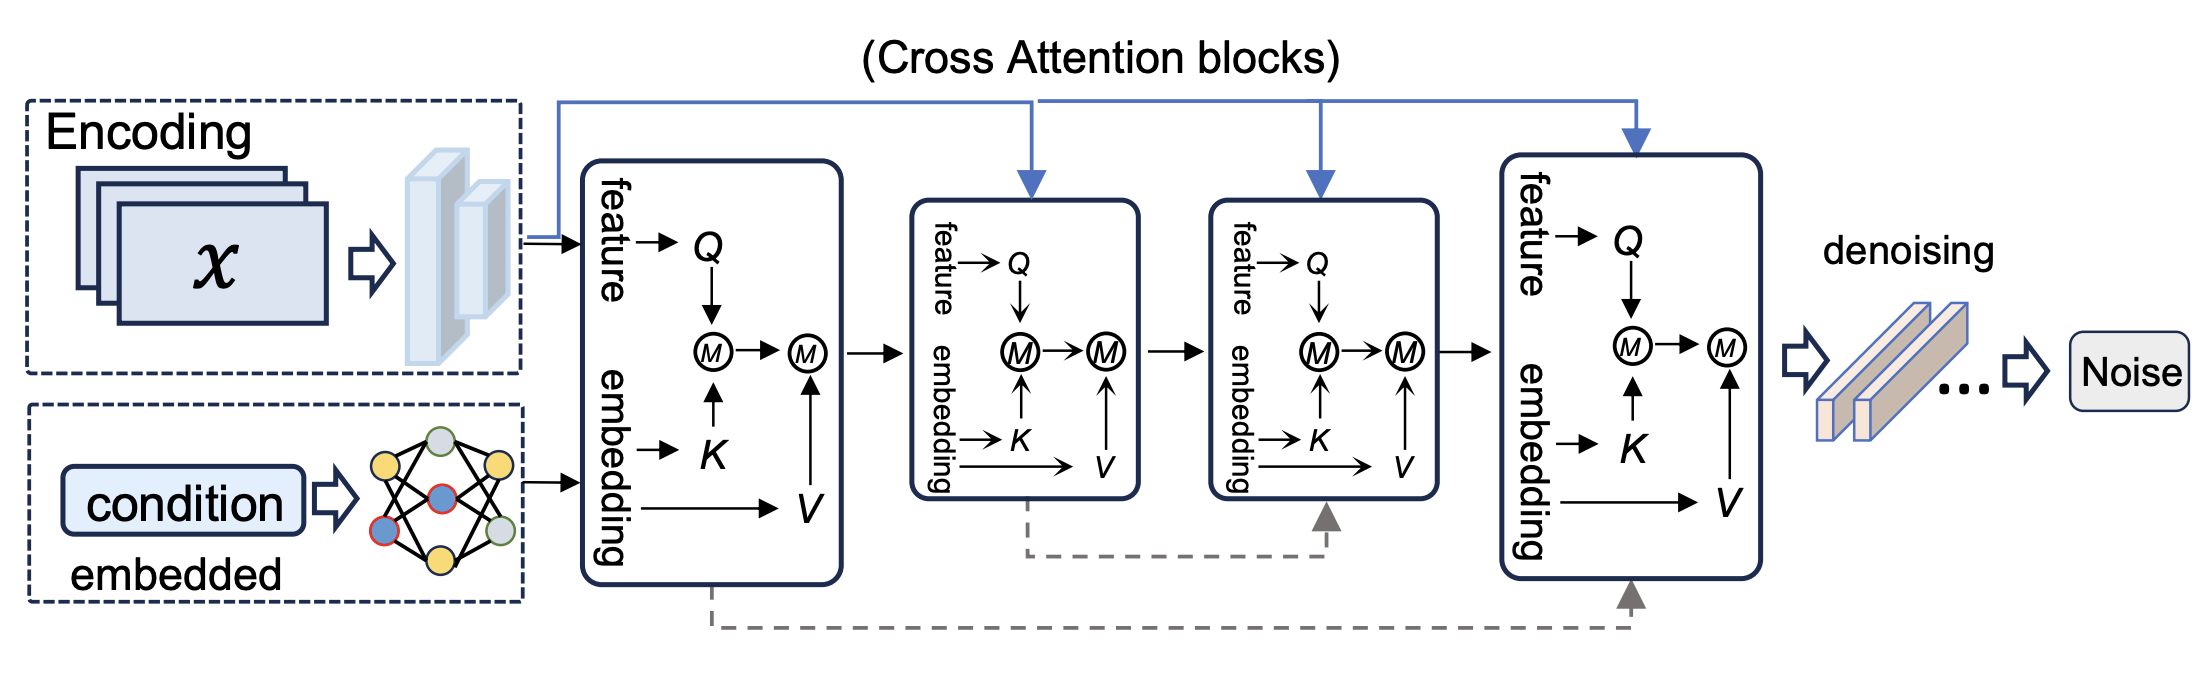
\includegraphics[width=0.6\textwidth]{images/diffusion_models/stable_diffusion/cross_attention.png}
    \caption{Cross-attention in Stable Diffusion. The $K,V$ matrices are derived from conditional embeddings, while the $Q$ matrix is projected from the image/noise encodings \cite{sun2024sora}.}
    \label{fig:cross_attention}
\end{figure}

Cross-attention aligns \textbf{two different sequences} by computing attention weights from a query sequence ($Q$) and applying them to key-value pairs ($K, V$). This mechanism is particularly effective in conditional generation tasks, such as text-to-image (T2I) and text-to-video (T2V), where text prompts guide the generation process.

In Stable Diffusion (Section~\ref{sec:stable_diffusion}), cross-attention is employed to condition the latent image encodings on text embeddings. Specifically, the input sequence $\textcolor{blue}{X}$ (e.g. images) is projected onto $Q$, while the conditional sequence $\textcolor{red}{Y}$ (e.g., text) is projected onto $K$ and $V$, using:

\begin{align*}
    Q = \textcolor{blue}{X}\cdot W_Q \\
    K = \textcolor{red}{Y}\cdot W_K \\
    V = \textcolor{red}{Y}\cdot W_V
\end{align*}

where $W_Q, W_K, W_V \in \mathbb{R}^{d \times d}$ are learnable projection matrices.

\textbf{Multi-head cross-attention} extends this by using multiple attention heads, each operating independently and concatenated together. Listing \ref{lst:stable_diffusion_cross_attention} shows a simplified PyTorch implementation of cross-attention.

\begin{lstlisting}[language=Python, caption={PyTorch implementation of cross-attention. The '@' operator represents the dot product.}, label={lst:stable_diffusion_cross_attention}]
class CrossAttention(nn.Module):
    def __init__(self, n_heads, d_embed, d_cross, 
                 in_proj_bias=True, out_proj_bias=True):
        super().__init__()
        self.q_proj = nn.Linear(d_embed, d_embed, bias=in_proj_bias)
        self.k_proj = nn.Linear(d_cross, d_embed, bias=in_proj_bias)
        self.v_proj = nn.Linear(d_cross, d_embed, bias=in_proj_bias)
        self.out_proj = nn.Linear(d_embed, d_embed, bias=out_proj_bias)
        self.n_heads = n_heads
        self.d_head = d_embed // n_heads

    def forward(self, x, y):
        # Projection and attention computation
        q = self.q_proj(x)
        k = self.k_proj(y)
        v = self.v_proj(y)
        
        weight = q @ k.transpose(-1, -2) / math.sqrt(self.d_head)
        weight = F.softmax(weight, dim=-1)
        output = weight @ v

        # Reshape and project output
        output = output.transpose(1, 2).contiguous()
        output = output.view_as(x)
        return self.out_proj(output)
\end{lstlisting}

The implementation is adapted from a \href{https://github.com/hkproj/pytorch-stable-diffusion/blob/e0cb06de011787cdf13eed7b4287ad8410491149/sd/attention.py#L100C1-L110C28}{re-implementation of Stable Diffusion}. Note that the official implementation contains a more \href{https://github.com/CompVis/stable-diffusion/blob/21f890f9da3cfbeaba8e2ac3c425ee9e998d5229/ldm/modules/attention.py#L152}{complex version of cross-attention}.

Notice lines 14, 15, 16 in listing \ref{lst:stable_diffusion_cross_attention}: the input $\textcolor{blue}{X}$ is projected onto $Q$ only, and $\textcolor{red}{Y}$ is projected onto both $K$ and $V$.














\subsection{Axial attention}

Axial attention \cite{axial_attention}, used in VideoGPT \cite{videogpt}, addresses the quadratic complexity of self-attention ($O(n^2)$) by attending to one axis at a time, reducing the complexity to $O(n\sqrt{n})$. Instead of processing the full input sequence, it alternately attends to masked rows and columns, saving computations while preserving global spatial context.

\begin{figure}
    \centering
    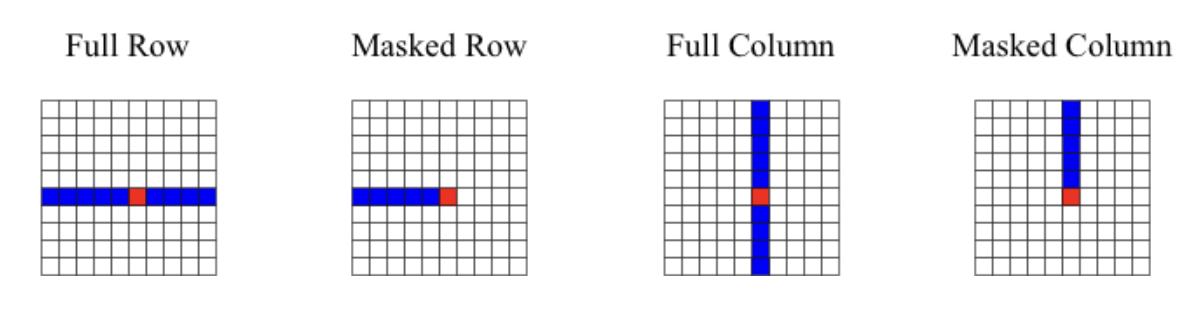
\includegraphics[width=0.6\textwidth]{images/appendix/attention/axial.png}
    \caption{Types of axial attention layers which are the building blocks of axial transformer.}
    \label{fig:axial_attention}
\end{figure}

This axial attention masking can be seen in figure \ref{fig:axial_attention}. The order of pixels that are from top-left to bottom-right and as an autoregressive pixel prediction model, which uses axial attention, will be predicting the pixel $p_{i, j}$ and not $p_{i+1, j}$ or $p_{i, j+1}$, which depends only on previous pixels.

Although axial transformer is not attending to every pixel, it still captures spatial global context more efficiently.
